\chapter{メールサーバへの接続フィルタリング}

メールサーバは、不特定多数のクライアント、あるいはメールサーバからの接続を受けます。
必要な接続、正規のユーザからの接続であれば問題はありません。
ですが、spam等の送信目的での接続や、サービスを提供しているユーザ以外からの接続は拒絶したいというのが一般的な考え方です。

本章では、そのための接続フィルタリングについて説明し舞う。

\section{クライアントからの接続フィルタリング}

もともと、メールを送受信するホストは、全てメールサーバでした。
あるときは他のメールサーバからの接続を受け、自分のスプールに、他のメールサーバ宛のメールがあれば、クライアントとしてサーバに接続し、メールを転送します。

現在のメールサービスには、メールサーバにメール転送を依頼するクライアントという存在があります。
クライアントは、SMTPによる通信は行いますが、メールの中継は行いません。
そのため、クライアントからの接続は、そのクライアントが利用できる権利のあるメールサーバに限り許可して、他のドメインへのメール転送は、メールサーバだけが行う、という形態になっています。

その、クライアントからの接続をフィルタリングするための方法について説明をします。


\subsection{OP25B}

\begin{figure}[htbp]
	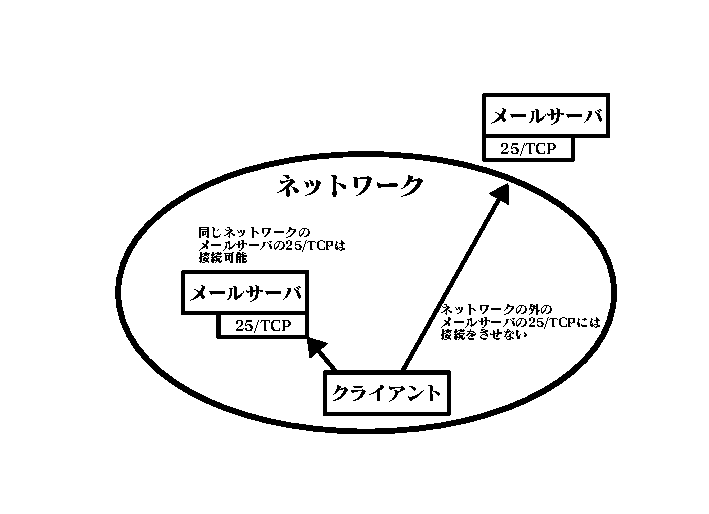
\includegraphics[width=12cm,clip]{draw/op25b.pdf}
	\caption{OP25B}
	\label{fig:op25b}
\end{figure}

メールサーバへの接続をフィルタリングする古典的な手法として、OP25B(Outbound Port 25 Blocking)というものがあります。
これは、図\ref{fig:op25b}のように、クライアントに対して、クライアントが接続されたネットワークの外のメールサーバの、25/TCPに接続させない、というフィルタリングを行う、メールセキュリティ手法です。
メールサーバに対しての設定でなく、ネットワークの出口でフィルタリングを行うという点に注意してください。
そして、これは自組織のメールサーバを守るものというより、他所のメールサーバに自組織のユーザが迷惑をかけないために行うものとなります。

インターネットサービスプロバイダがメールサービスを提供するとき、メールサーバへの接続は25/TCP、つまりSMTPのポートを使用していました。
これは、クライアントからの接続もサーバ間のメール転送も、おなじ25/TCPで行っていた、ということです。
そのため、25/TCPはどこからでも接続できるように開放する必要があります。
そして、目的とするサーバの25/TCPに接続することで、第三者への転送を行わないとしても、そのサーバが管理するメールボックスに、直接メールを送り込むことはできてしまいます。

昔のことですが、メールサーバは誰でもどこからでも接続して使えるものでした。
そのため、ネットワークの外のメールサーバの25/TCPへの接続を禁止することで、互いに第三者のメールサーバの利用を防ぐようにしました。
これが、OP25Bというメールセキュリティです。

実際の運用では、ISPが、インターネット接続サービスを利用しているユーザに対して、自分の提供する以外のメールサーバへの接続ができないように、インターネットへの出口でフィルタリングを行います。

この方法は、外部のメールサーバへの、クライアントからの接続を禁止するというものです。一見するとこれで全て解決しそうですが、ユーザが別のネットワークからメールサーバを利用できない句なる、という欠点があります。
OP25Bを行いつつ、他のネットワークからメールサーバを利用したいというユーザの利便性を確保するのが、Pop Before SMTPやSMTP-AUTHです。

\subsection{OP25Bが設定されていないネットワーク}

OP25Bは、メールサーバ側でなく、ネットワーク化の管理者が自主的に行うものです。
そのため、OP25Bが行われていないネットワークも多くあります。
ISPが固定回線の一般ユーザに接続サービスを提供している場合は、プロバイダ側でOP25Bが設定されていることが多いです。
とはいえ、一般ユーザ向けの接続で、OP25Bを行っていないISPも多くあります。

また、例えば法人向けなど、インターネット接続に制限をされていないことが前提の接続サービスもあります。
この場合、OP25Bは接続サービスを受ける側のネットワーク管理者が行うかどうかを選択できます。

そのため、OP25Bがされていないネットワークからの接続を制限する方法として、後述するS25Rとグレイリスティングの組み合わせが出てきました。

\subsection{POP before SMTP}

POP Before SMTP(PbS)は、POPの認証に成功したホストから、メールサーバへの25/TCPへの接続を、一定時間許可するという方法です。
SMTP-AUTHの普及で、2019年現在は、あまり使用されなくなっています。

PbSによる認証は、メールサーバへのPOP3接続によって行われます。
POP3はユーザ認証を含むプロトコルなので、それをメール転送についても利用します。
一度POPでの認証に成功したホストは、その後、、サーバの設定に依存する一定時間、MTAへのアクセスが許可されます。
正確に表現すると、POP出の認証に成功したホストのIPアドレスからメールサーバへの接続が一定時間きょかされる、ということです。

このPbSですが、重大な欠点があります。
それは、認証がホスト単位で行われるということです。
PbSは認証に成功した、という情報だけを利用します。そのため、次回以降のメールサーバとの接続では、PbSに成功したユーザかどうか、という判定はされません。
そして、接続許可はIPアドレス単位、つまり、メールサーバから見えるIPアドレス単位で行われます。

つまり、IPv4でNATを使用している環境では、インターネット側から見えるIPアドレスが同じであれば接続が許可されるということです。
これは、NATの背後にあるネットワークの全てのホストからノ接続が、一定時間の間、許可されるということでもあります。

そのため、セッション単位での認証を行えるSMTP-AUTHが普及したことで、PbSは利用されることが減っています。

\subsection{SMTP-AUTH}

SMTP-AUTHは、クライアントがサーバに接続する、セッション毎に認証を行います。
そのため、現在ではクライアントがメールサーバに接続する際の認証として、最も使われているものです。

SMTP-AUTHは、SMTPを拡張したものですが、SMTPそのものが認証機能を持っているわけではありません。
SASL(Simple Authentication and Security Layer)という、アプリケーション層のプロトコルに認証機能を追加するアプリケーションで認証をします。
SMTP-AUTHは、SMTPのセッションの中で認証情報を取得し、SASLに送ります。
そして、判定結果を返してもらいます。メールサーバでは、SASLによる認証結果をもって、そのセッションでメール転送を行うかを決定します。

SMTP-AUTHの利点は、SMTPのセッション単位で認証を行なうことです。そのため、NATの背後にあるクライアントからの接続でも、特定することができます。
欠点は、SASLのデーモンがメールサーバと別に必要になることと、認証のためのユーザデータベースが必要となることです。

SASLとメールサーバは独立したデーモンとなります。そのため、認証系を別のインスタンスに置くことで、負荷分散を刷ることが可能です。
また、認証のためのユーザデータベースは、POPやIMAPで用いるものと共用することができます。
SMTP-AUTHを利用するときのユーザデータベースのは、LDAPやRDBMSで構築することが多くなります。
そのユーザデータベースは、ローカルメールボックスの一覧、SMTP-AUTH、POP3、IMAPの認証系の全てで利用可能なように属性を設定します。

さて、ここまで、SMTP-AUTHでメール転送時に認証を行う、という説明しました。
ですが、OP25Bが設定されているネットワークの中からでは、そもそも外部のメールサーバに接続することができません。
そこで、SMTP-AUTHを行うためのポートが設定されました。それが、Submissionポートです。

\subsection{Submission}

SMTP-AUTHは、クライアントとメールサーバの間のセッションについて、認証を行います。
そうすることで、クライアントがインターネットのどこから接続してきていても、そのメールサーバを利用する権利があるユーザであることを確認することができます。
ですが、OP25Bのため、そもそもメールサーバに接続することができません。

そのため、SMTP-AUTHによる任所を行う場合専用のポートが設定されました。それが、Submissionという通称のついたポートです。
ポート番号表記で、587/TCPになります。

SubmissionポートはOP25Bの対象外であるため、ほとんどの場合、インターネット経由で接続可能です。
また、Submissionポートは平文、もしくは、StartTLSによる保護のいずれかで接続されます。
これは、サーバ側の設定によって、平文での通信が許可されるか、StartTLSによるTLSへの移行が強制されるかが異なります。

\subsection{SMTPS}

SMTP-AUTHで使用するポートは、もうひとつSMTPSとよばれる、465/TCPがあります。
このポートは、元々は暗黙的TLSで通信を保護するSMTPである、SMTPSに割り当てられたWell-Known Portです。
ですが、SMTP-AUTHの通信を暗黙的TLSで保護する通信のために利用されています。

SMTPSも、OP25Bの対象外であるため、インターネット経由で接続することができます。
当然ながら、SMTPSでは、TCPのハンドシェイク後、TLSのセッションを開始した後にSMTPのセッションを開始するほうの通信が強制されます。

\subsection{SubmissionとSMTPSの使い分け}

\begin{figure}[htbp]
	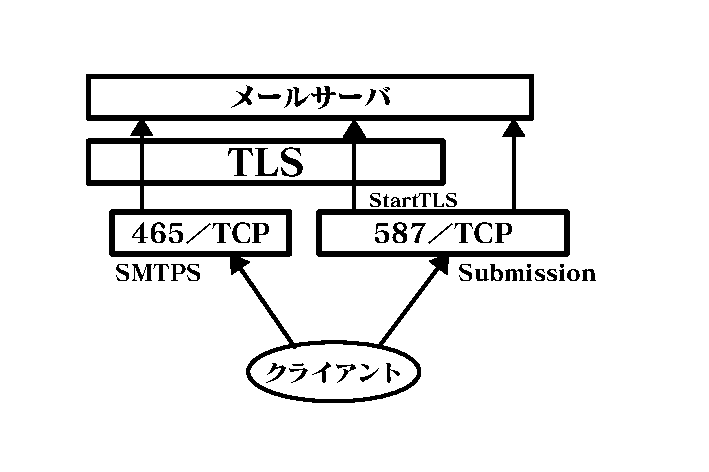
\includegraphics[width=12cm,clip]{draw/withtls.pdf}
	\caption{SubmissionとSMTPS}
	\label{fig:submission_smtps}
\end{figure}

SubmissionとSMTPSは、SMTP-AUTHのクライアント・サーバ間通信に使うことは同じです。
違いは、TLSが明示的であるか暗黙的であるか、という点です。
この関係は、図\ref{fig:submission_smtps}としてあらわされます。

Submissionは、TLSに対応していないメールクライアントでも接続可能な設定とすることができます。
この時、サーバ側ではStartTLSでTLSのセッションに移行しなくても、セッションを許可する設定をします。
ただし、平文で情報が流れることを許可することでもあるので、セキュリティ綿では弱くなります。

SMTPSは、TLSのセッションの上で、メールサーバとクライアントの通信が行われます。
そのため、通信が最初から最後まで保護される、という利点があります。
また、SMTPのセッション開始前に、TLS証明書の検証による、接続先サーバの真性検証が可能であるという利点があります。
SubmissionはStartTLSの後でないと、証明書の検証ができません。

ただ、TLSに遷移した後は、機能はどちらも変わらないため、SubmissionとStattTLSによる接続のみ提供し、SMTPSは提供しない事例もあります。


\section{S25Rとグレイリスティング}

メールサーバでは、Submissonポート、SMTPSポートを提供したとしても、SMTPの25/TCPは全てのホストに対して開いておく必要があります。
インターネットで接続してくるメールサーバに対応するためではありますが、これは、OP25Bが施されていない全てのネットワークからの接続が可能になる、ということです。
そのため、OP25Bが設定されていないネットワークから、宛先ドメインのメールサーバに直接接続して、spamを送り込むという手法が発生しました。
その対策として考案されたのが、S25Rであり、S25Rを拠り適切に適用する手段としての、グレイリスティングとの組み合わせです。

\subsection{メールサーバへの接続をどのように選択するか}

メールサーバは、メールの転送を受け、そのメールが自分のメールボックス宛でなければ他のメールサーバに転送します。
25/TCPへの転送は、メールサーバでなくても可能です。
そして、ほとんどのメールサーバで、25/TCPに届いたメールが自分の管理するメールボックス宛であれば、それをメールボックスに保存します。
つまり、spamの送信を意図したとき、宛先のメールサーバに直接接続してメールを送りつける、という方法を使うことができます。

プロバイダなどのメールサーバを経由しないのは、送出されるメールのspamフィルタリングや送信データ量の制限を回避するためです。
また、DNSのMXレコードで、そのドメインのメールサーバは公開されています。そのため、直接目標のサーバに接続して、効率的にspamを送りつけることができる、という理屈です。

\subsection{RBL}

S25Rについて説明する前に、古典的な接続フィルタリング手法であるRBL(Realtime Blackhole List)について説明します。

RBLは、DNSの仕組みを利用して、接続してきたホストがspamの送信元であるかを判定します。
spamを送信していたなど、メールサーバとして好ましくない動作をしていたホストをレコードに記載します。
メールサーバは接続してきたホストのIPアドレスを、RBLに問い合わせます。
もし、そのホストのがRBLに登録されていば、DNSと同じ仕組みで、レコードが返されます。

RBLは、誰でも無償で使えるものと、セキュリティベンダが収集した情報を元にレコード登録を行っているものとがあります。
前者は誰でもエントリを登録できるようになっていることがあります。
この、誰でも登録できるRBLでは、、間違いや嫌がらせなどで、問題の無いメールサーバが登録される可能性があり、それが欠点となっています。
また、RBLにレコードが登録されていないIPアドレスについては、全く判定をすることができません。

これらの理由から、フォルスポジティブ、フォルスネガティブのどちらも発生しやすいという欠点があります。
ですが、確実にspma送信元と判っているIPアドレスからの接続を排除することができるので、実運用で信用できるRBLを利用するのがよいでしょう。

\subsection{S25R}

S25Rとは、Se;ective SMTP Rejectionの略称です。
途中に25文字あるという意味ではなく、SMTPに対して適用する、という意味で、ポート番号から25を取っています。

S25Rは、接続元の逆引き情報を用いて、メールサーバへの接続を許可するかどうかを判定する方法です。
簡単に説明すると、まず、逆引きができないホストからの接続は、接続拒否します。
次に、プロバイダがユーザに割り当てるIPアドレスの逆引きが可能な場合、ホスト名が一定のパターンに収まることが多い、という特徴があります。
そのパターンは正規表現で記述できるため、それに一致したものは、メールサーバでない何かからの接続である、と判断して接続を拒否します。
たとえば、ISPが一般ユーザに割り当てるIPアドレスに付けたホスト名は、そのIPアドレスを含む、などです。

S25Rは、メールサーバでないホストから、つまり、メールサーバに直接接続してspamを送り込もうとするクライアントからの接続を拒否することができる、有用な方法です。
ですが、S25Rには、メールサーバとして許可すべきものを弾いてしまう、フォルスポジティブの問題があります。
セキュリティで情報を与えないために、わざと逆引きのレコードを登録しないポリシーの運用をしている組織が挙げられます。
また、ISPか接続サービスで複数IPアドレスの割り当てを受けるとき、逆引き委譲には、別途申請が必要二なることが多いです。
ユーザレベルでのDNS運用の練度経験が減少しつある現在、逆引きができない、という一点で接続してくるホストを排除することは危険ですらあります。

\subsection{グレイリスティング}

前述したような、S25Rのフォルスポジティブ問題を解決しつつ、さらにメールサーバの選別をより高い精度で行うのが、グレイリスティングです。

グレイリスティングは、グレイリストという一覧を使います。では、グレイリストとは何なのでしょうか。
ネットワークで接続制限を行うとき、接続許可対象の一覧をホワイトリスト、接続拒否対象の一覧をブラックリストと呼びます。
ホワイトリストに載っているところからの接続のみ許可し、他を拒絶するのがホワイトリスト方式です。
逆に、ブラックリストに載っているところからの接続のみ拒否し、他を拒絶するのが、ブラックリスト方式になります。

グレイリストは、疑わしいが接続を一時的に許可する、という意味で、ホワイトリストとブラックリストの中巻という意味合いがあります。
まず、接続してきたホストについて、S25Rで判定を行います。
もし、そのホストがS25Rに引っかかった場合は、グレイリストに載っていれば接続を許可します。
グレイリストに載っていなければ、リザルトコード450の、Temporary Errorを返して接続拒否します。
、
グレイリストに載る条件は、接続を拒否されてから時間をおいて再度接続をしてきた場合です。
SMTPの規格では、何らかの原因で宛先のメールサーバへの接続ができなかった場合、5分の間隔をおいてリトライすることになっています。
正しくメールサーバとして動くメールサーバであれば、このリトライ動作を行うはず、というのがグレイリスティングの考え方です。

また、グレイリストは、一定時間が経過すると、そのエントリを消去します。

この方法で、DNSに逆引きエントリを持たないメールサーバからの接続をフォローすることができます。
また、spam送信目的でメールサーバに接続するホストのほとんどは、再接続を試みません。
再接続の試行には、メールキューへの貯留が必要になり、リソースを拠り多く必要とするためです。


